\chapter{Recommender Systems and Social Networks}
\label{c:recommendersystemsandsocialnetworks} This chapter is dedicated to the introduction of the relevant theoretical concepts that need to be understood in order to properly understand social recommender systems. It is arranged in three sections: The first section gives an overview over recommender systems' history, application areas and theoretical concepts. The second section is devoted to social networks and properties that are important for the incorporation of information into recommender systems. The third section then combines the two fields by introducing ways to incorporate social network information into recommendations, thus creating social recommender systems.

\section{Recommender Systems}
\label{st:recommendersystems} People face the challenge of making decisions and weighing different options every day. Often they take into consideration not only their own opinion and knowledge, but also the advice and recommendations of others. But these methods have their limits. A user might for example never hear about a good book that he would really like, if none of his friends knows that book. And often the almost infinite number of alternatives (e.g. what movie to watch or what music to listen to) makes it impossible to properly evaluate all options and find the best one. This is where a computer-based system can outperform human recommendations. Recommender systems are tools that try to predict the valuation users have for different items. They aim at helping the user in his decision-making processes, like what items to buy, what movies to watch or what music to listen to. Advantages over human recommendations include the much larger set of recommenders (even people who do not know a user personally might contribute some valuable information), the more systematical inclusion of a user's history and his already expressed preferences and the possibility to computationally deal with a much larger amount of alternatives. The possible application space of recommender systems is endless and there exist real-world examples in many different areas like books, restaurants, financial services \cite{Felfernig_2007} or even persons (online dating).

There are a lot of factors that determine the goodness and the practical success of recommender systems. Different application areas demand different abilities. In some areas, speed might be the crucial factor, in others transparency might be critical (users want to know how the recommendations are made), or it might be the case that users want a very broad range of new items recommended instead of only very similar ones. In reality, recommender systems are often used in commercial settings and the design of a particular recommender system should be highly dependent on the environment where it will be used. It is important to carefully evaluate the requirements posed by the environment and build the recommender system according to those requirements.
\newline

As a consequence of the various conditions and surroundings recommender systems operate in, there exist many different approaches and recommendation techniques. \cite{Ricci_2011} give a good overview over existing methods and algorithms. Here, two of the most popular approaches are described, while the focus of the experiments lies explicitly on the collaborative filtering approach.

\subsection{Content-based Filtering}
\label{sst:contentbasedfiltering} Content-based filtering looks at the similarity between different items. Based on the attributes and characteristics of items a user has rated in the past, the system will recommend new items with similar characteristics to the user. If someone has watched a lot of action movies with Sylvester Stallone (and given them a good rating), it is likely that movies starring Sylvester Stallone or movies belonging to the action genre will be recommended to this person. Whereas in movies one often has to make appropriate categorizations manually, this process can be automated with text-based content (like books or webpages). Text can be scanned for frequently used keywords and recommendations can be made based on keyword frequency.

\subsubsection{Challenges}
\label{ssst:challenges} There are numerous challenges to this approach. One that was already mentioned before is the categorization of items. Where content is not text-based, it is hard to automatically extract information about the content, especially in movie or music domains. Another problem is the new-user problem: It is hard to provide accurate recommendations for new users who have only rated very few items so far, since there is not much information about their preferences. Furthermore, there exists also the danger of over-specialization, which means that the user from the Sylvester Stallone example might never be recommended a comedy movie if he has not watched one yet, even though he might actually like it.

\subsection{Collaborative Filtering}
\label{sst:collaborativefiltering} The method of collaborative filtering does not use any information about items' characteristics in order to make predictions. Instead it takes into account the rating history of all users. This new approach already addresses one of the big challenges of content-based methods, that is the high categorization-cost. The new-user problem still exists, but is less severe.

In user-based collaborative filtering, the idea is to find users with similar rating behaviour and predict ratings for an item based on these similar users' ratings for this item. Item-based collaborative filtering tries to find items that have been rated similarly across all users and then makes a prediction for an item based on the user's ratings for similar items.

\subsubsection{Formal Framework}
\label{ssst:formalframework} To mathematically describe the different algorithms and metrics that are used in the experiments, a formal framework is introduced here. Let $U = \{1,...,u\}$ denote the set of users and let $G = \{1,...,g\}$ denote the set of items. Let $r_i(j)$ denote the actual rating of user $i \in U$ for item $j \in G$. The ultimate task for every recommender system is to find a good estimate $\hat{r}_i(j)$ for an item $j$ that user $i$ has not rated yet. The closer $\hat{r}_i(j)$ is to the user's actual rating $r_i(j)$ (which exists even if the user has not explicitly rated the item yet; it should be seen as the actual valuation of the user for that item), the more accurate the recommendation is.

As mentioned above, there exist many aspects that contribute to the quality of a recommender system and the performance might be highly dependent on the environment the system operates in. Nevertheless, accuracy is considered to be the most important metric to measure the performance of a recommender system. One common measure to express the accuracy is the \textit{root-mean-square error} (RMSE). For a series of $n$ predictions $\hat{r}_n$ and actual ratings $r_n$, it is defined as follows:

\begin{equation}
RMSE = \sqrt{\frac{1}{n} \sum_{i=1}^{n}(r_n - \hat{r}_n)^2}
\label{eq:rmse}
\end{equation}

\subsubsection{User-based Collaborative Filtering}
\label{ssst:userbasedcf} User-based collaborative filtering tries to find users that are similar to a particular user. The assumption is that similar users will be good predictors for the estimation of $\hat{r}_i(j)$. The first step is thus to find a measure of similarity between two users. There exist different measures, of which two commonly used ones will be presented.

\subsubsection{Pearson Correlation Coefficient}
\label{ssst:pearsoncorrelationcoefficient} The Pearson correlation coefficient measures the similarity between two users $i$ and $i'$. Let $\bar{r}_i$ denote the average rating over all items user $i$ has rated so far. $G_{ii'}$ ist the set of items both users have already rated. Then the Pearson correlation coefficient is calculated as follows:

\begin{equation}
sim(i,i') = \frac{\sum_{j \in G_{ii'}}{(r_i(j)-\bar{r}_i)(r_{i'}(j)-\bar{r}_{i'})}}{\sqrt{\sum_{j \in G_{ii'}}{(r_i(j)-\bar{r}_i)^2}}\sqrt{\sum_{j \in G_{ii'}}{(r_{i'}(j)-\bar{r}_{i'})^2}}}
\label{eq:pearson}
\end{equation}

The pearson correlation coefficient results in a similarity value between $-1$ and $+1$.

\subsubsection{Cosine Similarity}
\label{ssst:cosinesimilarity} A second similarity measure that is widely used to calculate how similar two users are is the cosine similarity. The cosine similarity calculates the similarity of orientation of two vectors. The two vectors $x_i$ and $x_{i'}$ in this case are the rating vectors of users $i$ and $i'$ respectively, containing all ratings $r_{i}(j)$ and $r_{i'}(j)$ respectively of the items in set $G_{ii'}$. The cosine similarity is then calculated as follows:

\begin{equation}
sim(i,i') = \frac{\sum_{j \in G_{ii'}}{r_{i}(j)\cdot r_{i'}(j)}}{\sqrt{\sum_{j \in G_{ii'}}{{r_{i}^2}(j)}}\sqrt{\sum_{j \in G_{ii'}}{{r_{i'}^2}(j)}}}
\label{eq:cosine}
\end{equation}

The similarities calculated with \eqref{eq:cosine} also lie in the range from $-1$ to $+1$.
\newline

Once all similarities $sim(i,i')$ for a user $i$ are calculated, the other users can be sorted by their similarity to user $i$. It makes sense to only consider the most similar users for the prediction of $\hat{r}_i(j)$, since their ratings correlate the most with user $i$'s ratings. The next step is thus to choose an appropriate subset of all users $i'$, which is called the \textit{neighbourhood} $N$ of a user. The size of this neighbourhood can be determined in different ways, it can either be a certain number (e.g. 50) or it can be determined through applying a threshold on the similarities (e.g. only include users with similarity greater than 0.5).

Once this neighbourhood set is determined, there exist different ways to compute the estimated rating $\hat{r}_i(j)$. We consider two approaches and a third one that combines the first two.

\subsubsection{Weighted Sum}
\label{ssst:weightedsum} The weighted sum aggregation takes into account that more similar users should have a bigger influence on the prediction than less similar ones. To predict rating $\hat{r}_i(j)$, the rating for item $j$ of each user $i'$ in the determined neighbourhood $N$ is weighted with $sim(i,i')$:

\begin{equation}
\hat{r}_i(j) = \frac{\sum_{i' \in N}{sim(i,i')\cdot r_{i'}(j)}}{\sum_{i' \in N}{sim(i,i')}}
\label{eq:weightedsum}
\end{equation}

\subsubsection{Adjusted Sum}
\label{ssst:adjustedsum} A problem that the weighted sum aggregation does not take into account is that users might interpret the rating scale differently. Some users might generally give lower ratings than others. To account for this, the adjusted sum prediction uses the average rating $\bar{r}_{i'}$ of each user $i'$.

\begin{equation}
\hat{r}_i(j) = \bar{r}_i + \frac{\sum_{i' \in N}{r_{i'}(j)\cdot \bar{r}_{i'}}}{\mid N\mid}
\label{eq:adjustedsum}
\end{equation}

\subsubsection{Adjusted Weighted Sum}
\label{ssst:adjustedweightedsum} The adjusted weighted sum combines both aspects; it weighs the users' ratings by their similarity and it adjusts the ratings with the average ratings:

\begin{equation}
\hat{r}_i(j) =  \bar{r}_i + \frac{\sum_{i' \in N}{sim(i,i')\cdot (r_{i'}(j) - \bar{r}_{i'})}}{\sum_{i' \in N}{sim(i,i')}}
\label{eq:adjustedweightedsum}
\end{equation}

Note that in all three approaches the sum is over all users in neighbourhood $N$. One has to take into account the fact that it is not certain that all users in $N$ have already rated item $j$. In fact, the sparser the rating matrix, the higher the probability that there are users who have not rated item $j$ and are therefore left out of the prediction calculation. The actual set of neighbours that influence $\hat{r}_i(j)$ can therefore be much smaller than $\lvert N \rvert$.

\subsubsection{Item-based Collaborative Filtering}
\label{ssst:itembasedcf} A different approach is item-based collaborative filtering. Instead of finding users with similar rating behaviour, this method looks for similarities between items. In contrast to content-based methods, no information about the actual content of the items is needed, but instead the rating profiles of the items across all users are considered. If a set of items similar to item $j$ can be found, the ratings user $i$ has given those items can be used to estimate $\hat{r}_i(j)$.

\subsubsection{Challenges}
\label{ssst:challengescf} As already mentioned, some of the main challenges of content-based filtering can be avoided with this approach, however there occur other, new challenges. The main difficulty with collaborative filtering can be the extremely high computational cost. Calculating all user- or item-similarities can be a serious issue, especially in domains with thousands of users and possibly millions of items.

\subsection{Related work}
\label{sst:rsrelatedwork} There is a vast variety of studies and papers that give a survey on the topic of recommender systems. \cite{Ricci_2011} give a good overview over existing approaches to recommender systems and explain in detail different properties of recommender algorithms. A recommender algorithm can be evaluated and compared to others with respect to these properties. By far the most used property to assess the quality of a recommender algorithm is its prediction accuracy. Since recommender algorithms aim at providing recommendations to users, it is safe to assume that users prefer algorithms that have a high prediction accuracy, that is they predict ratings that are close to the actual rating of a user.

\cite{Adomavicius_2005} describe the state-of-the-art of recommender algorithms and give theoretical background on content-based, collaborative filtering and hybrid approaches. They further suggest possible extensions to enhance these algorithms.

\section{Social Networks}
\label{s:socialnetworks} Social networks are structures that have existed for a very long time. It is even safe to say that people would not be able to live by themselves, without any social connections. There exist many kinds of social ties between people, including friendships, family, or also work-related relationships. A social network is basically made up of two components; the social actors (which often are people, but could also be organizations or other social entities) and the ties between those actors.

Whereas in the past social network structures were often implicitly present, but hard to explicitly capture and analyze, the rise of the internet and the effects of globalization are responsible for the appearance of online social networks like Facebook or Twitter. These networks often are a good reflection of real social networks, with the big advantage that they can be empirically studied and analyzed.

Social networks can be mathematically represented by graphs. A graph consists of a set of nodes $N$ and a set of edges $E$ which are dyadic links between two nodes. Graphs are often drawn with nodes as little circles and edges as connecting lines between the circles. The edges can either be undirected, meaning that the relationship is bi-directional, or they can be directed (drawn as arrows instead of lines) meaning that the relation goes only in one direction.

\begin{figure}[!ht]
\centering
\begin{minipage}[b]{5 cm}
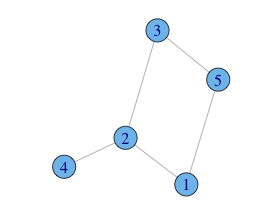
\includegraphics[width=150px]{./2-recommendersystemssocialnetworks/figures/SampleGraph.png}
\label{f:simplegraph}
\end{minipage}
\begin{minipage}[b]{5 cm}
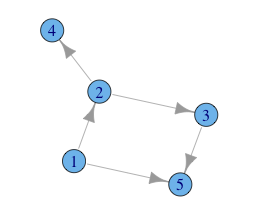
\includegraphics[width=150px]{./2-recommendersystemssocialnetworks/figures/SampleGraph2.png}
\label{f:simplegraph}
\end{minipage}
\caption[An undirected and a directed graph, each with 5 nodes and 5 edges.]
{An undirected and a directed graph, each with 5 nodes and 5 edges.}
\end{figure}

In the space of online social networks, a Twitter graph would be a directed graph because you can follow a person without this person following you. The Facebook social network would be represented as an undirected graph, since friendships are always bi-directional. For this thesis, we will only consider two-way friendships and thus we will always work with undirected graphs. Edges can also be weighted, with the weight of an edge indicating the strength of the tie between two nodes. This aspect is also beyond the scope of this thesis and edges will not be weighted, or in other words will all have the same weight 1.

\subsection{Graph notions and properties}
\label{sst:graphproperties} Once an existing social network is transformed into its mathematical representation, a graph, we can analyze different properties of this graph in order to find out more about the structure of the network. Different properties of a graph are presented and also properties that are characteristic for real-world social networks will be explained. This will play a big role in the graph generation section, where the task is to generate networks with realistic social network properties.

\textbf{Degree:} The degree of a node is the number of edges adjacent to it. In a social network where edges represent friendships the degree is the number of friends someone has.

\textbf{Distance:} The distance between two nodes is the number of edges of the shortest path between those two nodes. A path is a sequence of edges that connect a sequence of nodes, and the shortest path between two nodes is the path that connects those two nodes through the least number of edges. In a social network where edges represent friendships between people, all your direct friends would thus have distance 1 from you, and friends of your friends would have distance 2.

\textbf{Average path length:} The average path length is the average length of the shortest paths of all possible node pairs. It is an indicator of how well information or data can be transported through a network. A shorter average path length means that information will spread across the network faster.

\textbf{Global clustering coefficient/Transitivity:} The clustering coefficient of a graph (also called transitivity) measures the tendence of nodes to cluster together and form cliques. A clique is a set of nodes where every node is connected to every other node. The clustering coefficient is defined as $\frac{3\:\times\:number\:of\:triangles}{number\:of\:connected\:triples}$, where a triangle is 3 nodes all connected with each other (a clique of size 3) and a connected triple is 3 nodes where at least one node is connected with both other nodes.

There also exists a local clustering coefficient which measures how close one node's neighbours are to being a clique.
\newline\newline
These are 4 basic and very important graph properties. They can help to categorize graphs and to find typical patterns in certain categories of networks. 

\subsection{Related Work}
\label{sst:snrelatedwork}

\section{Social Recommender Systems}
\label{st:socialrecommendersystems}

\subsection{Social Collaborative Filtering}
\label{sst:socialcf}